\chapter{Podsumowanie}
\label{chap:results}

	Niniejszy rozdział dokonuje podsumowania rezultatów prowadzonej pracy. Prezentuje wyniki testów, które przeprowadzono w celu weryfikacji spełnienia wymagań. Porównuje szacunki dotyczące poboru mocy z rzeczywistym poborem. Ponadto dokonuje oceny bezpieczeństwa oraz responsywności systemu.

    \section{Testowanie}

        Tabela \ref{tbl:tests} przedstawia przeprowadzone testy oraz ich wyniki.

        \begin{table}[h!]
            \caption{Testy wymagań}
            \centering
            \begin{subtable}[c]{\textwidth}
                \centering
                    \begin{tabular}{|p{2cm}|p{2,5cm}|p{9,5cm}|}
                    \hline
                    TEST\_1               & \multicolumn{2}{l|}{\textbf{Poprawność procesu autoryzacji}} \\ \hline
                    \cellcolor[gray]{0.8} Wymaganie             & \multicolumn{2}{p{12cm}|}{FNRQ\_1 Kontrola dostępu do pomieszczeń, FNRQ\_8 Sygnalizacja przyznania lub odmowy dostępu} \\ \hline
                    \cellcolor[gray]{0.8} \multirow{2}{*}{Opis} & Przebieg           & Zbliżenie się do zamka, przyłożenie identyfikatora upoważnionego do uzyskania dostępu do zamka. \\ \cline{2-3} 
                    \cellcolor[gray]{0.8}                      & Oczekiwany wynik   & Układ zamka informuje o pomyślnej decyzji.                                                 \\ \hline
                    \cellcolor[gray]{0.8} Wynik                 & \multicolumn{2}{p{12cm}|}{Pozytywny - układ zamka informuje o pomyślnej decyzji.}                                                                                  \\ \hline
                    \end{tabular}%
                \label{tbl:test1}
                \vspace{10mm}
            \end{subtable}
        \quad%
            \begin{subtable}[c]{\textwidth}
                \centering
                    \begin{tabular}{|p{2cm}|p{2,5cm}|p{9,5cm}|}
                    \hline
                    TEST\_2               & \multicolumn{2}{l|}{\textbf{Poprawność procesu autoryzacji}}                                                            \\ \hline
                    \cellcolor[gray]{0.8} Wymaganie             & \multicolumn{2}{p{12cm}|}{FNRQ\_1 Kontrola dostępu do pomieszczeń, FNRQ\_8 Sygnalizacja przyznania lub odmowy dostępu}                                                                                    \\ \hline
                    \cellcolor[gray]{0.8} \multirow{2}{*}{Opis} & Przebieg           & Zbliżenie się do zamka, przyłożenie identyfikatora nieupoważnionego do uzyskania dostępu do zamka. \\ \cline{2-3} 
                    \cellcolor[gray]{0.8}                      & Oczekiwany wynik   & Układ zamka informuje o niepomyślnej decyzji.                                                 \\ \hline
                    \cellcolor[gray]{0.8} Wynik                 & \multicolumn{2}{p{12cm}|}{Pozytywny - układ zamka informuje o niepomyślnej decyzji. Przetestowano z użyciem dwóch kart RFID oraz jednego breloka RFID.}                                                                                  \\ \hline
                    \end{tabular}%
                \label{tbl:test2}
                \vspace{10mm}           
            \end{subtable}
        \quad%
            \begin{subtable}[c]{\textwidth}
                \centering
                    \begin{tabular}{|p{2cm}|p{2,5cm}|p{9,5cm}|}
                    \hline
                    TEST\_3               & \multicolumn{2}{l|}{\textbf{Poprawność zapisu i podglądu historii dokonanych prób dostępu}}                                                            \\ \hline
                    \cellcolor[gray]{0.8} Wymaganie             & \multicolumn{2}{p{12cm}|}{FNRQ\_2 Przeglądanie historii prób dostępu do pomieszczeń}                                                                                    \\ \hline
                    \cellcolor[gray]{0.8} \multirow{2}{*}{Opis} & Przebieg           & Dokonanie próby dostępu zakończonej sukcesem. Dokonanie próby dostępu zakończonej porażką.                                    \\ \cline{2-3} 
                    \cellcolor[gray]{0.8}                      & Oczekiwany wynik   & Próby dostępu zakończone sukcesem i porażką zapisane w bazie danych.                                                 \\ \hline
                    \cellcolor[gray]{0.8} Wynik                 & \multicolumn{2}{p{12cm}|}{Pozytywny - próby dostępu zakończone sukcesem i porażką zapisane w bazie danych. Możliwy podgląd danych z aplikacji zarządzającej.}                                                                                  \\ \hline
                    \end{tabular}%
                \label{tbl:test3}
                \vspace{10mm}           
            \end{subtable}
            \label{tbl:tests}
        \end{table}
    
        \pagebreak  

        \begin{table}[h!]
            \ContinuedFloat
            \caption{Testy wymagań, c.d.}
            \begin{subtable}[c]{\textwidth}
                \centering
                    \begin{tabular}{|p{2cm}|p{2,5cm}|p{9,5cm}|}
                    \hline
                    TEST\_4               & \multicolumn{2}{l|}{\textbf{Poprawność dodawania identyfikatorów}}                                                            \\ \hline
                    \cellcolor[gray]{0.8} Wymaganie             & \multicolumn{2}{p{12cm}|}{FNRQ\_3 Dodawanie identyfikatorów, FNRQ\_4 Przeglądanie identyfikatorów powiązanych z danym zamkiem, FNRQ\_6 Dostęp do grupy pomieszczeń za pomocą jednego identyfikatora }                                                                                    \\ \hline
                    \cellcolor[gray]{0.8} \multirow{2}{*}{Opis} & Przebieg           & Dodanie identyfikatora za pomocą menu w aplikacji GUI, wraz z wyborem zamków, do których będzie upoważniony.  \\ \cline{2-3} 
                    \cellcolor[gray]{0.8}                      & Oczekiwany wynik   & Identyfikator oraz powiązania z zamkami zapisane w bazie danych.                                                 \\ \hline
                    \cellcolor[gray]{0.8} Wynik                 & \multicolumn{2}{p{12cm}|}{Pozytywny - identyfikator oraz powiązania z zamkami zapisane w bazie danych. Możliwy podgląd danych z aplikacji zarządzającej.}                                                                                  \\ \hline
                    \end{tabular}%
                \label{tbl:test4}
                \vspace{10mm}           
            \end{subtable}
        \quad%
            \begin{subtable}[c]{\textwidth}
                \centering
                    \begin{tabular}{|p{2cm}|p{2,5cm}|p{9,5cm}|}
                    \hline
                    TEST\_5               & \multicolumn{2}{p{12cm}|}{\textbf{Poprawność blokowania dostępu do pomieszczenia dla żądanego identyfikatora}}                                                            \\ \hline
                    \cellcolor[gray]{0.8} Wymaganie             & \multicolumn{2}{p{12cm}|}{FNRQ\_5 Blokowanie dostępu do pomieszczeń dla wybranego identyfikatora }                                                                                    \\ \hline
                    \cellcolor[gray]{0.8} \multirow{2}{*}{Opis} & Przebieg           & Usunięcie powiązania identyfikatora z zamkiem za pomocą przycisku w aplikacji GUI.  \\ \cline{2-3} 
                    \cellcolor[gray]{0.8}                      & Oczekiwany wynik   & Żądane powiązanie usunięte z bazy danych. Dostęp za pomocą żądanego identyfikatora do żądanego zamka niemożliwy.                                                 \\ \hline
                    \cellcolor[gray]{0.8} Wynik                 & \multicolumn{2}{p{12cm}|}{Pozytywny - żądane powiązanie usunięte z bazy danych. Dostęp za pomocą żądanego identyfikatora do żądanego zamka niemożliwy.}                                                                                  \\ \hline
                    \end{tabular}%
                \label{tbl:test5}
                \vspace{10mm}           
            \end{subtable}
        \quad%
            \begin{subtable}[c]{\textwidth}
                \centering
                    \begin{tabular}{|p{2cm}|p{2,5cm}|p{9,5cm}|}
                    \hline
                    TEST\_6               & \multicolumn{2}{p{12cm}|}{\textbf{Dostęp do pomieszczenia za pomocą grupy identyfikatorów}}                                                            \\ \hline
                    \cellcolor[gray]{0.8} Wymaganie             & \multicolumn{2}{p{12cm}|}{FNRQ\_7 Dostęp do pomieszczenia za pomocą grupy identyfikatorów }                                                                                    \\ \hline
                    \cellcolor[gray]{0.8} \multirow{2}{*}{Opis} & Przebieg           & Dodanie dwóch identyfikatorów za pomocą aplikacji GUI. Dodanie upoważnienia do tego samego zamka przy obu identyfikatorach.  \\ \cline{2-3} 
                    \cellcolor[gray]{0.8}                      & Oczekiwany wynik   & Dwa powiązania zapisane w bazie danych. Obu identyfikatorom przyznawany jest dostęp.                                                 \\ \hline
                    \cellcolor[gray]{0.8} Wynik                 & \multicolumn{2}{p{12cm}|}{Pozytywny - dwa powiązania zapisane w bazie danych. Obu identyfikatorom przyznawany jest dostęp.}                                                                                  \\ \hline
                    \end{tabular}%
                \label{tbl:test6}
                \vspace{10mm}           
            \end{subtable}
            \label{tbl:tests}
        \end{table}
    
        \pagebreak  

        \begin{table}[h!]
            \ContinuedFloat
            \caption{Testy wymagań, c.d.}
            \begin{subtable}[c]{\textwidth}
                \centering
                    \begin{tabular}{|p{2cm}|p{2,5cm}|p{9,5cm}|}
                    \hline
                    TEST\_7               & \multicolumn{2}{l|}{\textbf{Czas pracy układu zamka na zasilaniu bateryjnym}}                                                            \\ \hline
                    \cellcolor[gray]{0.8} Wymaganie             & \multicolumn{2}{p{12cm}|}{XXRQ\_1 Długość czasu pracy układu zamka na baterii równa minimum 1 rok }                                                                                    \\ \hline
                    \cellcolor[gray]{0.8} \multirow{2}{*}{Opis} & Przebieg           & Placeholder.  \\ \cline{2-3} 
                    \cellcolor[gray]{0.8}                      & Oczekiwany wynik   & Placeholder                                                 \\ \hline
                    \cellcolor[gray]{0.8} Wynik                 & \multicolumn{2}{p{12cm}|}{Placeholder.}                                                                                  \\ \hline
                    \end{tabular}%
                \label{tbl:test6}
                \vspace{10mm}           
            \end{subtable}
        \quad%
            \begin{subtable}[c]{\textwidth}
                \centering
                    \begin{tabular}{|p{2cm}|p{2,5cm}|p{9,5cm}|}
                    \hline
                    TEST\_7               & \multicolumn{2}{l|}{\textbf{Czas odpowiedzi układu zamka}}                                                            \\ \hline
                    \cellcolor[gray]{0.8} Wymaganie             & \multicolumn{2}{p{12cm}|}{XXRQ\_2 Czas odpowiedzi układu zamka nie dłuższy niż 3 sekundy }                                                                                    \\ \hline
                    \cellcolor[gray]{0.8} \multirow{2}{*}{Opis} & Przebieg           & Placeholder.  \\ \cline{2-3} 
                    \cellcolor[gray]{0.8}                      & Oczekiwany wynik   & Placeholder                                                 \\ \hline
                    \cellcolor[gray]{0.8} Wynik                 & \multicolumn{2}{p{12cm}|}{Placeholder.}                                                                                  \\ \hline
                    \end{tabular}%
                \label{tbl:test6}
                \vspace{10mm}           
            \end{subtable}
            \label{tbl:tests}
        \end{table}

    \section{Wydajność energetyczna}

        Założono, że w wyniku prób dostępu lub przypadkowych wzbudzeń czujnika zbliżeniowego, układ zamka zostaje wybudzony około 120 razy w ciągu doby, z czego za każdym razem pozostaje w stanie operacyjnym od 7 do maksymalnie 16 sekund. Oznacza to że układ przez ponad 98\% czasu pozostaje w stanie uśpienia, co świadczy o tym, że pobór prądu w tym stanie będzie miał dominujący wpływ na ogólną efektywność energetyczną. Na podstawie wykonanych pomiarów, można oszacować dobowy pobór prądu na około 107 mAh. Stosując 9 ogniw galwanicznych o napięciu wyjściowym 1.5 V i pojemności 1100 mAh, połączonych zgodnie ze schematem przedstawionym na rysunku \ref{fig:battery_layout}, można zapewnić stałe źródło zasilania o napięciu 4.5V i pojemności 3300 mAh. W takiej konfiguracji żywotność układu wynosi w przybliżeniu 30 dni.

        Powodem tak niskiej żywotności jest wysoki pobór prądu w stanie spoczynku. Odpowiedzialny za tą nieefektywność jest element układu zasilania wykorzystanej płytki prototypowej: regulator napięcia LD1117. Jego standardowy prąd spoczynkowy wynosi około 5 mA~\cite{AMS1117-ds}. Zastępując go regulatorem AP2112K o prądzie spoczynkowym w granicach 50 μA~\cite{AP2112K-ds}, można zredukować pobór prądu w stanie uśpienia z 4 mA do około 150 μA, tym samym zwiększając żywotność.

        \begin{figure}[]
            \centering
            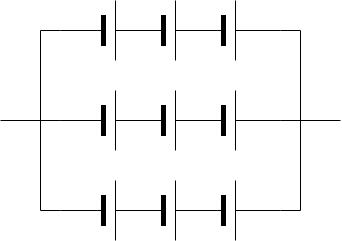
\includegraphics[width=0.5\textwidth]{chapters/images/battery_layout.png}
            \caption{Schemat połączenia baterii}
            \label{fig:battery_layout}
        \end{figure}


	\textbf{Wydajność energetyczna - TBD}

	\textbf{Responsywność - TBD}

	\textbf{Bezpieczeństwo - TBD}

	\section{Możliwe rozszerzenia}

        W ramach niniejszej pracy stworzony został prototyp rozwiązania. Niektóre planowane funkcjonalności nie zostały zaimplementowane ze względu na ograniczenia czasowe i budżetowe. Pozostawiono jednak możliwość rozbudowy systemu. Poniżej przedstawiono kilka problemów, których system w obecnym stanie nie adresuje, wraz z możliwymi rozwiązaniami.

        \subsection{Mechanizm wyjścia}

            Opisywane rozwiązanie nie obejmuje implementacji mechanizmu opuszczenia strefy chronionej systemem kontroli dostępu. W zależności od potrzeb końcowego użytkownika, możliwe rozwiązanie to montaż dodatkowego czytnika po przeciwnej stronie drzwi i połączenie go z kontrolerem wejścia w przypadku gdy wymagana jest obustronna kontrola dostępu bądź zastosowanie przycisku którego naciśnięcie powoduje zwolnienie zamka w przypadku gdy wymagana jest tylko kontrola wejścia do chronionego obszaru.

        \subsection{Obsługa większej liczby zamków}

            W celu umożliwienia obsługi przez system liczby zamków przekraczającej 1, wystarczająca byłaby modyfikacja podsystemu autoryzacji w taki sposób, aby mógł on obsługiwać równoległe żądania od klientów.

        \subsection{Wygodna konfiguracja parametrów sieci}

            W obecnej implementacji dane dostępu do sieci (nazwa sieci oraz hasło) zostały zagnieżdżone w oprogramowaniu konrolera. Zmniejsza to elastyczność konfiguracji urządzenia, wymagając jego przeprogramowania za każdym razem gdy zmianie ulegnie nazwa lub klucz dostępu do sieci.

            Możliwym rozwiązaniem tego problemu byłaby implementacja trybu konfiguracji. Tryb ten powodowałby przejście kontrolera w tryb Access Point przy zachowaniu dwóch warunków: (1) nastąpiło uruchomienie, a nie wybudzenie z trybu głębokiego uśpienia oraz (2) na określonym wejściu pojawił się stan wysoki. Przejście kontrolera w tryb Access Point umożliwiłoby udostępnienie prostego interfejsu webowego, za pomocą którego administrator systemu mógłby wprowadzić niezbędne do działania dane, takie jak nazwa sieci, hasło, a także adres IP i numer portu serwera autoryzacji. Aby zachować wysoki poziom bezpieczeństwa, komunikacja pomiędzy urządzeniem administratora i kontrolerem powinna odbywać się przy wykorzystaniu protokołu TLS.

        \subsection{Sygnalizacja stanu baterii}

            W obecnym stanie system nie implementuje mechanizmów informowania serwera o swoim stanie energetycznym.
            Sygnalizacja stanu baterii umożliwiłaby administratorowi systemu bieżące monitorowanie wszystkich zamków objętych systemem oraz szybką reakcję w przypadku, gdy baterie wymagałyby wymiany. Modyfikacja ta wymagałaby uzyskania dostępu do danych na temat naładowania baterii przez mikrokontroler oraz przesyłania ich okresowo do serwera, najlepiej w momentach, gdy jest on już wybudzony z powodu wykrycia ruchu w jego otoczeniu.

        \subsection{Obsługa kont użytkowników w podsystemie zarządzania}
            Podsystem zarządzania nie implementuje mechanizmu dostępu do zasobów, co czyni system mniej bezpiecznym. W końcowym produkcie należałoby rozszerzyć go o możliwość tworzenia kont użytkowników i przypisywania im określonych uprawnień co do odczytu i zapisu danych.

    \section{Podsumowanie}

        W ramach niniejszej pracy stworzono funkcjonalny prototyp systemu, który po odpowiednich modyfikacjach miałby szansę efektywnej pracy w odpowiednim środowisku.

        Dzięki wykorzystaniu zdalnego serwera do przeprowadzenia procesu uwierzytelniania system zapewnia większą elastyczność i łatwość zarządzania niż alternatywne systemy wykorzystujące zamki pracujące w sposób autonomiczny.

        Rozwiązanie cechuje się wygodą montażu, ponieważ nie wymaga przewodów zasilających i komunikacyjnych prowadzonych w ścianach budynków. Przy wdrażaniu rozwiązania nie jest konieczna modyfikacja istniejącej infrastruktury budynku, z wyjątkiem wymiany samych zamków. System nie wymaga żadnych dodatkowych komponentów sprzętowych poza zamkami i serwerem.

        Wydajność energetyczna podsystemu sterowania zamkiem została osiągnięta przez zarządzanie zasilaniem jego peryferiów oraz kontrolę stanu zasilania mikrokontrolera w celu minimalizacji poboru mocy i maksymalizacji czasu pracy na zasilaniu bateryjnym.

        Bezpieczeństwo systemu na wielu poziomach zapewnia wykorzystanie mechanizmów takich jak TLS w warstwie komunikacji pomiędzy zamkiem a serwerem czy szyfrowanie pamięci Flash w warstwie operacji na danych w mikroprocesorze w układzie zamka.